% !TEX root = ../thesis.tex
% !TEX spellcheck = en-US

\clearpage

\section{Exploration}
\label{sec:Exploration}

The first part of this thesis project is dedicated to the exploration of the problem space. Driven by the research objectives the goal was twofold: At once to find an approachable yet challenging research problem in the context of data from a recruitment platform while, simultaneously evaluating the potential for creating value through an enhanced user experience or new use cases for the service. The exploration is divided into a discovery phase and a definition phase where the problem scope is first diverging and then converging respectively. These phases will be described in the following sections.

\subsection{Discovery Phase: Exploring the Problem Scope}
\label{Discovery Phase: Exploring the Problem Scope}

During the discovery phase the problem space was first opened up through exploration of user needs and initial field research better understand the problem context. Additionally literature research and benchmarking of approaches helped getting a picture of related scientific work. It should be noted though that quantitative user research was rather minimal due to time constraints and the scientific nature of this thesis.

Initially a set of interviews with stakeholders from Product Management to Marketing and Engineering who work with the product as well as potential users helped obtaining a good understanding about the service offerings of a recruitment platform and the current trends in the industry. Exploring the various data that the platform generates, an important learning was that large parts of the data are in form of written language and much of it in a more or less unstructured way.

Exploration was therefore focused on language related problems. Literature research revealed a strong interest from the research community in tasks related language modeling using neural networks and other connectionist approaches that had gained traction through the latest advances of \gls{Deep Learning}. Several methods were then tested as quick prototypes, also leading to the learning that real data is often noisy and inconsistent. In addition ideas for focusing the problem search were evaluated, ranging from practical ideas such as predicting trends in the job marking to wilder ones such as digitalizing the complete Sanoma archive to analyze how written language evolves over time in order to predict when a text was written or to identify trending terms or even writing styles.

Through further experimentation, research and discussions the problem of utilizing the implicit knowledge in the main text body of job listings was deemed a good fit for further focus. It was both an interesting and challenging research problem and could potentially be of practical use, e.g. when identifying the requirements for a job inside this text or other applications. This decision set the course for the definition phase to begin with increased focus on narrowing explored set of problems to a single problem definition.

\subsection{Definition Phase: Framing the Problem}
\label{sub:Definition Phase: Framing the Problem}

The definition phase of the design process is characterized by explorative convergence of the problem space through iterative reframing and refinement of the problem definition, hand in hand with further experimentation and learning within the new scope. For this research project it is marked by three main decision points where the problem definition was reformulated.
These three iterations of converging towards a final problem definition are described next in terms of rationale for the chosen direction, the experimental approach to learn within this new scope and the results and learnings obtained.

\subsubsection{Inferring Structure of Job Advertisements}
\label{subs:Inferring Structure in Job Advertisements}


\paragraph{Rationale}
\label{par:Rationale}

During the discovery phase it became apparent that a there is large amounts of unstructured and implicit knowledge in the data of job advertisements. Specifically large portions of the data are natural language in relatively free form. One example for this which also makes up a significant amount of data is the text body of each job advertisement. This part, just like the content of a job listing in print media, contains all the information about a job position that a company wants to communicate to a potential applicant.

The contained information can be useful to provide better services, e.g.\ by inferring requirements for a job from the text in order to show more relevant listings to the user. Another potential application of machine learning to this data is to predict popularity within certain target audiences for advertisements, for instance to help recruiters design better job listings. In many cases it is useful for these applications to first better understand the structure and content of the job ad. Thus learning the structure of job advertisements was set as a subject of further study.


\paragraph{Experimental Approach}
\label{par:Experimental Approach and Metrics}

To learn how humans interpret structure and content of job ads and what they consider a good structural representation of the information contained a set of experiments was carried out. Five participants from various professional background were asked to highlight sections of the text in a job advertisement and to label these sections by describing what the section is about. Afterwards they were asked to restructure the job ad into a bullet-point list based on these highlighted sections.

No specific metrics were used as this prototype purely explorative to gain a basic understanding how terms like \emph{structure} and \emph{content} or \emph{topics} are interpreted and applied given the job listing samples. Each participant was provided with a \gls{Google Docs} document including one random job advertisement in English and the task was to first highlight parts they felt belonged to a certain part and then to structure these parts. The exact formulation was as follows:

\blockquote{Cheers for helping out with this little experiment for my thesis! My aim here is to find out how people would structure job ads to help find the relevant information faster.

You'll work with the job advertisement below. Your task is the following:
\begin{enumerate}
  \item First tag the job advertisement below into parts. Mark sections of it and use a word or two to categorize this section using the comment tool. You can tag the ad into sections however you want and even make the sections overlap. The goal here is to tag the content of the job ad that you think belongs to different categories, properties or topics. To tag the text, use the comment tool like this: ``We're looking for a Quality Buzzword Engineer.''
  \item Now fill the bullet-point list in the last section of this document with the tagged sections/categories/topics you found. It should roughly contain the same information as the ad but in a structured way using your tags. You can use sub-points categories if you want.
\end{enumerate}
In total try to spend no more than 30 minutes on this. Don't worry about it too much, the key is to just do it how it makes sense to you.}

A full example of this task as it was provided for the participants can be found in the Appendix in Section~\ref{sub:Understanding How Humans Structure Text}.

\paragraph{Results}
\label{par:Results}

After initially expressing difficulties with open and ambiguous task participants were provided with help by providing analogous examples (e.g.\ to label the description of a car and which parts talk about the components while others talk about the owner etc.). While this helped it was still perceived as a very difficult task as it leaves lots of room for interpretation.
The outcomes were quite various, especially along the following spectra:

\begin{itemize}
  \item Generality versus specificity: A section about the language requirements was labelled as \emph{Requirements} by one participant and a similar section as \emph{language requirements}
  \item Content versus structural elements: A heading was described in one instance as \emph{Job description} and a very similar one by another participant as \emph{Job description section indicator}
  \item Objectivity versus judgement: Some sections were judged by their content, e.g. as \emph{Empty words}
\end{itemize}

Also some participants built a nested structure in the second part of the task while others formulated rather wide areas to group the information in a flat list of topics.

\paragraph{Learnings and Conclusions}
\label{par:Learnings and Conclusions}

One meaningful learning was that also explorative experiments need to be constrained and well-defined as posing the question so openly lead to great difficulties understanding and performing it and to diffuse outcomes. Nevertheless it gave some initial insight in possible ways to capture and structure this type of texts in job advertisements and sparked discussions for the following research. Thus the problem of structuring job advertisements was set up for refinement through an experiment of larger scale.

\subsubsection{Multi-label Paragraph Classification}
\label{subs:Multi-label Paragraph Classification}

\paragraph{Rationale}
\label{par:Rationale}

The problem was of learning structure was broken down into three parts, namely 1) finding sections of text that form a functional unit, 2) identify a label that communicates the structural function of each such section and 3) inferring a hierarchy over possible labels and therefore also over the structure of the sections.

As each of these problems is a challenge of its own the focus was laid on finding the labels of sections while fixing the sections to be paragraphs and ignoring the possibility of a hierarchy of the labels. Based on these constraints a new experiment was set up where paragraphs were labelled by participants through a purpose-built web interface. The the aim was to collect a larger sample of data that would be better quantifiable, less biased and more varied through a higher number of participants, and to use this data for deepening the understanding of the problem and to evaluate the feasibility of tackling it with a first proof-of-concept prototype.


\paragraph{Crowd-sourced Data Collection}
\label{par:Crowd-sourced Data Collection}

To collect the data a tool was build, consisting of a \gls{Node.js} server using \gls{MongoDB} as a database and communicating via a JSON with a simple website front-end using the \gls{Mustache} template engine.
The tool was shared on social media and it's source code is publicly available on \gls{GitHub} (see Section~\ref{sub:thesis-tagger: A Tool for Tagging Chunked Job Ads} for a description and a pointer to the source code).

The data generated by using the free-form text description of each job ad and splitting it into paragraphs as can be seen in the software package as well\footnote{\url{https://github.com/cle-ment/thesis-tagger/blob/master/pre-processing.ipynb}}.

The exact task given to the participants was ``Describe what each section is about by adding one or more tags/keywords to it''. They were shown a job ad that was split into paragraphs and besides each paragraph was a text field to enter 1 or more tags as Figure~\ref{fig:thesis-tagger-interface} shows.

\begin{figure}[h]
  \centering
  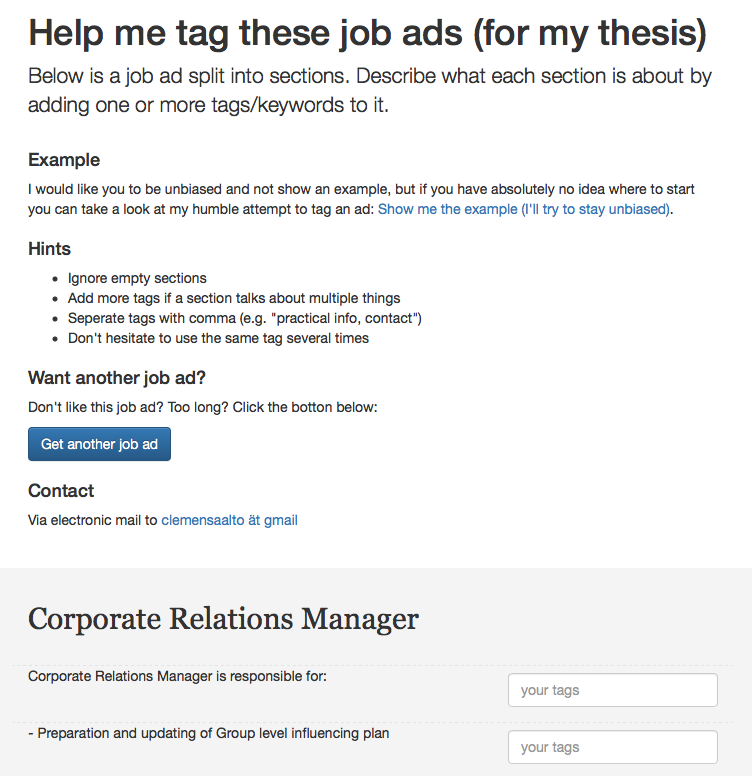
\includegraphics[width=\textwidth]{img/thesis-tagger-interface.png}
  \caption{Screen capture of the interface of the tagging tool}
\label{fig:thesis-tagger interface}
\end{figure}

In a first step the tool was only shown to 3 participants to get immediate feedback if the user interface had flaws and whether the task was understood. Based on this feedback the tool was improved by providing an example for the participants and then tested with a slightly larger group of 12 persons. After correcting a few minor details in the user interface a public link was then shared via social media and other channels with as many people as possible. A few days later the tool was then also shared internally within Sanoma where it was set up as a competition to tag the most possible job ads which greatly increased participation.

\paragraph{Experiments for Multi-label Paragraph Classification}
\label{par:Experiments for Multi-label Paragraph Classification}

To test whether automatic prediction of these obtained labels for paragraphs was possible a small prototype was build. For classification a TF.IDF weighed N-gram model was built that uses the word counts with the words associated with a label to create mappings for these labes in a common vector space (see Section~\ref{subs:N-gram Models} for details). Using this vector space we can then apply various classification algorithms with the assumption that closeness of labels in the vector space translates to similarity of the labels in the real world domain. Since every paragraph was potentially be labelled with multiple labels this problem was set up as multi-label classification where the absence or presence of each label is predicted for a paragraph. Several algorithms were applied, including \gls{kNN}, a Naive Bayes Classifier and Decision Trees (see Section~\ref{sub:Classification Methods using Vector Space Models} for details).

As expected this became very difficult as the data was extremely sparse with only a few cases of labels being assigned. The reason of course was that the choice of labels was completely left open and therefore most labels had only one paragraph associated with it.
To counter this problem the approach chosen was clustering the data once algorithmically and once manually.

Algorithmic clustering was carried out with using \gls{Lloyds Algorithm} for \gls{K-means clustering}, increasing the number of clusters and measuring the \gls{silhouette score} as a measure of how well clusters were separated. The silhouette score did not indicate a clear minimum at any point and the separation of clusters did not follow a trend. Figure~\ref{fig:kmeans_pca} s
hows an example of the clustering when assuming 6 and 8 clusters respectively and a visualization of the first principal components using \gls{PCA}.

\begin{figure}[h]
    \centering
    \begin{subfigure}[b]{1\textwidth}
        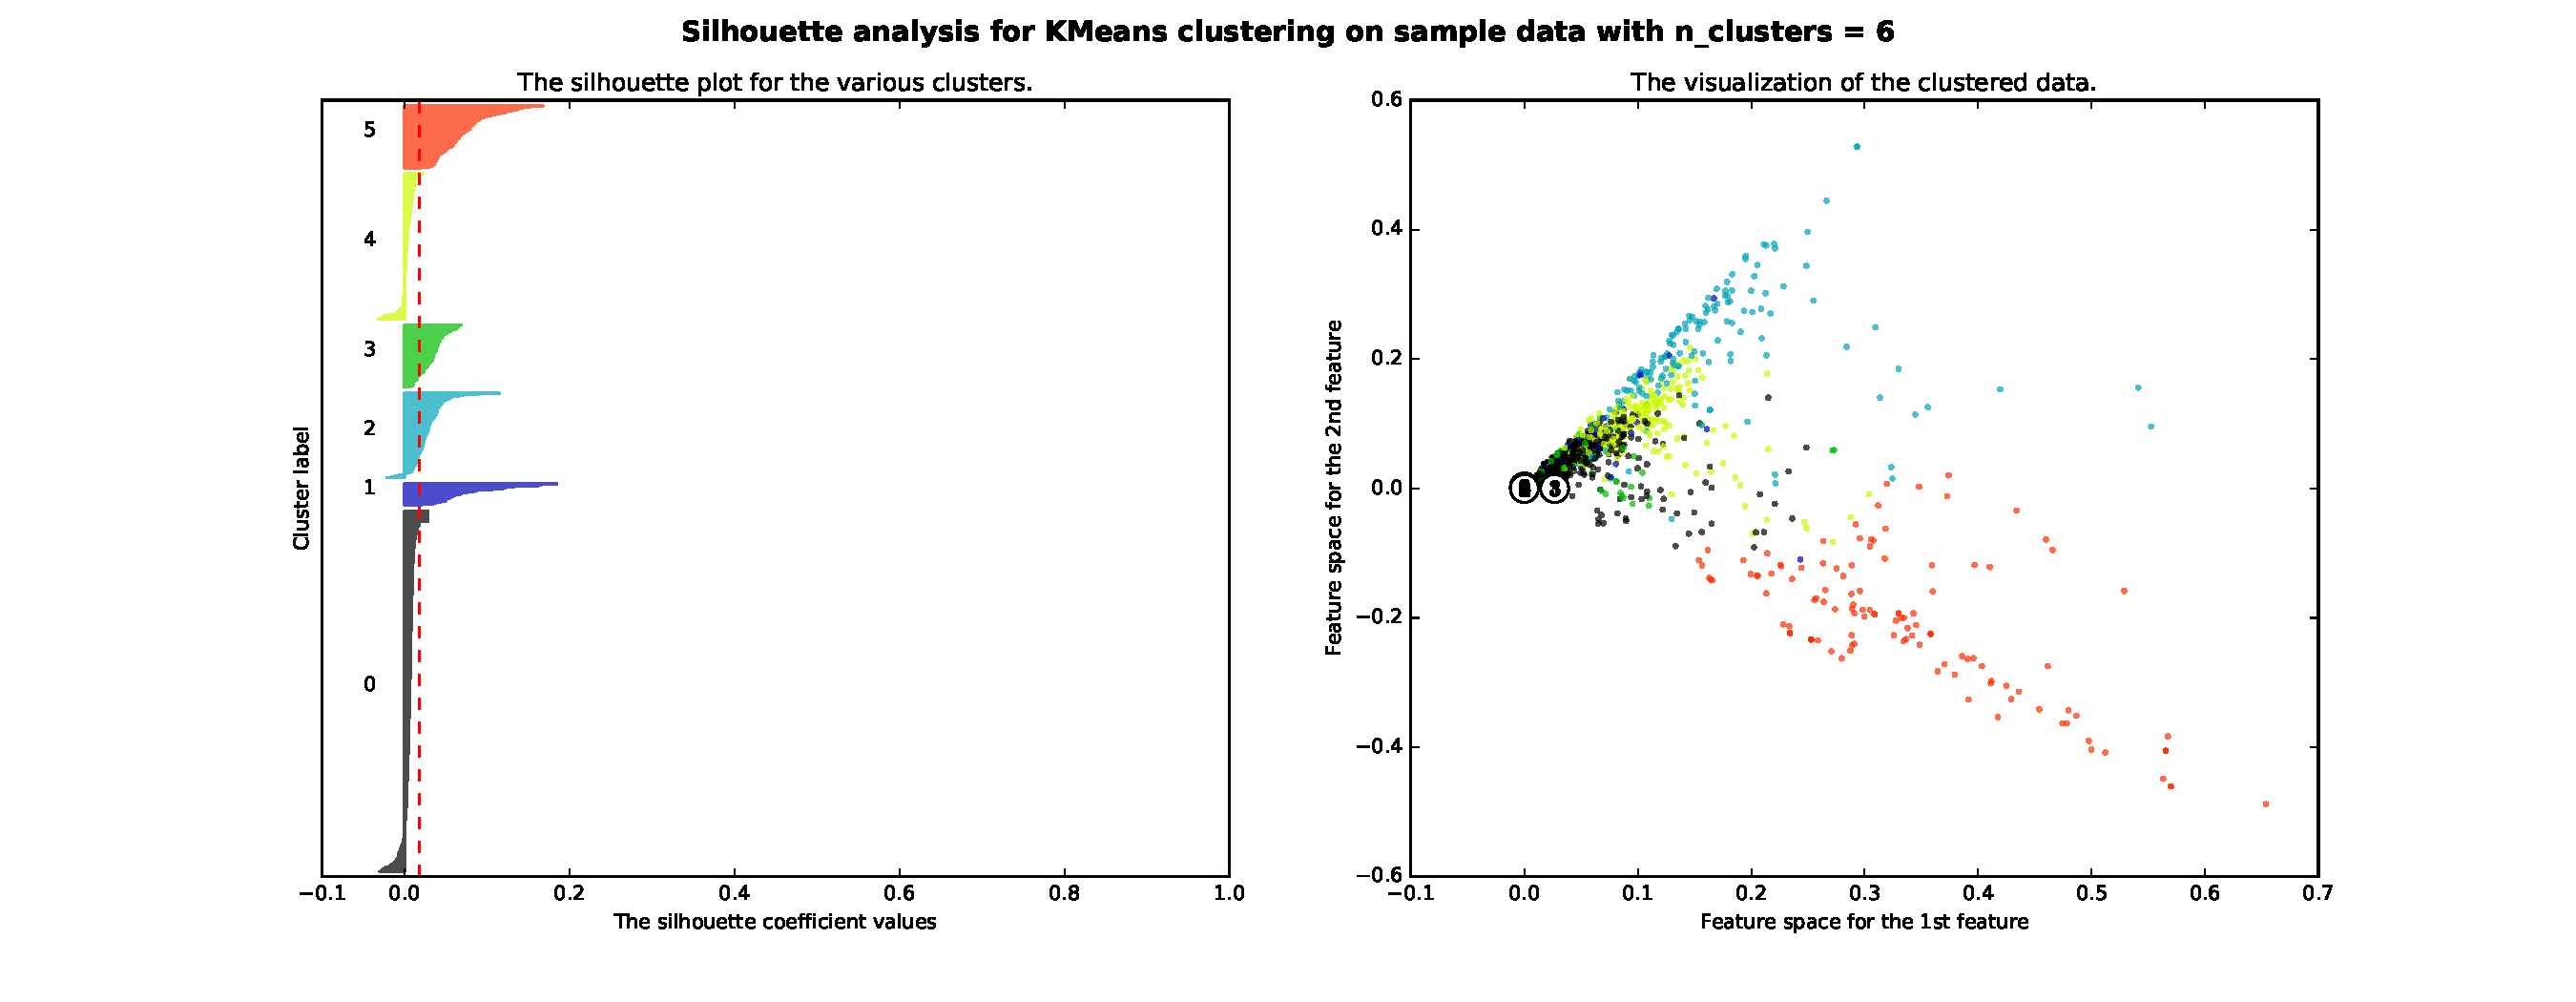
\includegraphics[width=1\textwidth]{img/exp-multi-label-paragraphs/kmeans_n=6_pca.pdf}
        \caption{Confidence}
\label{fig:kmeans_n=6_pca}
    \end{subfigure}
~
    \begin{subfigure}[b]{1\textwidth}
        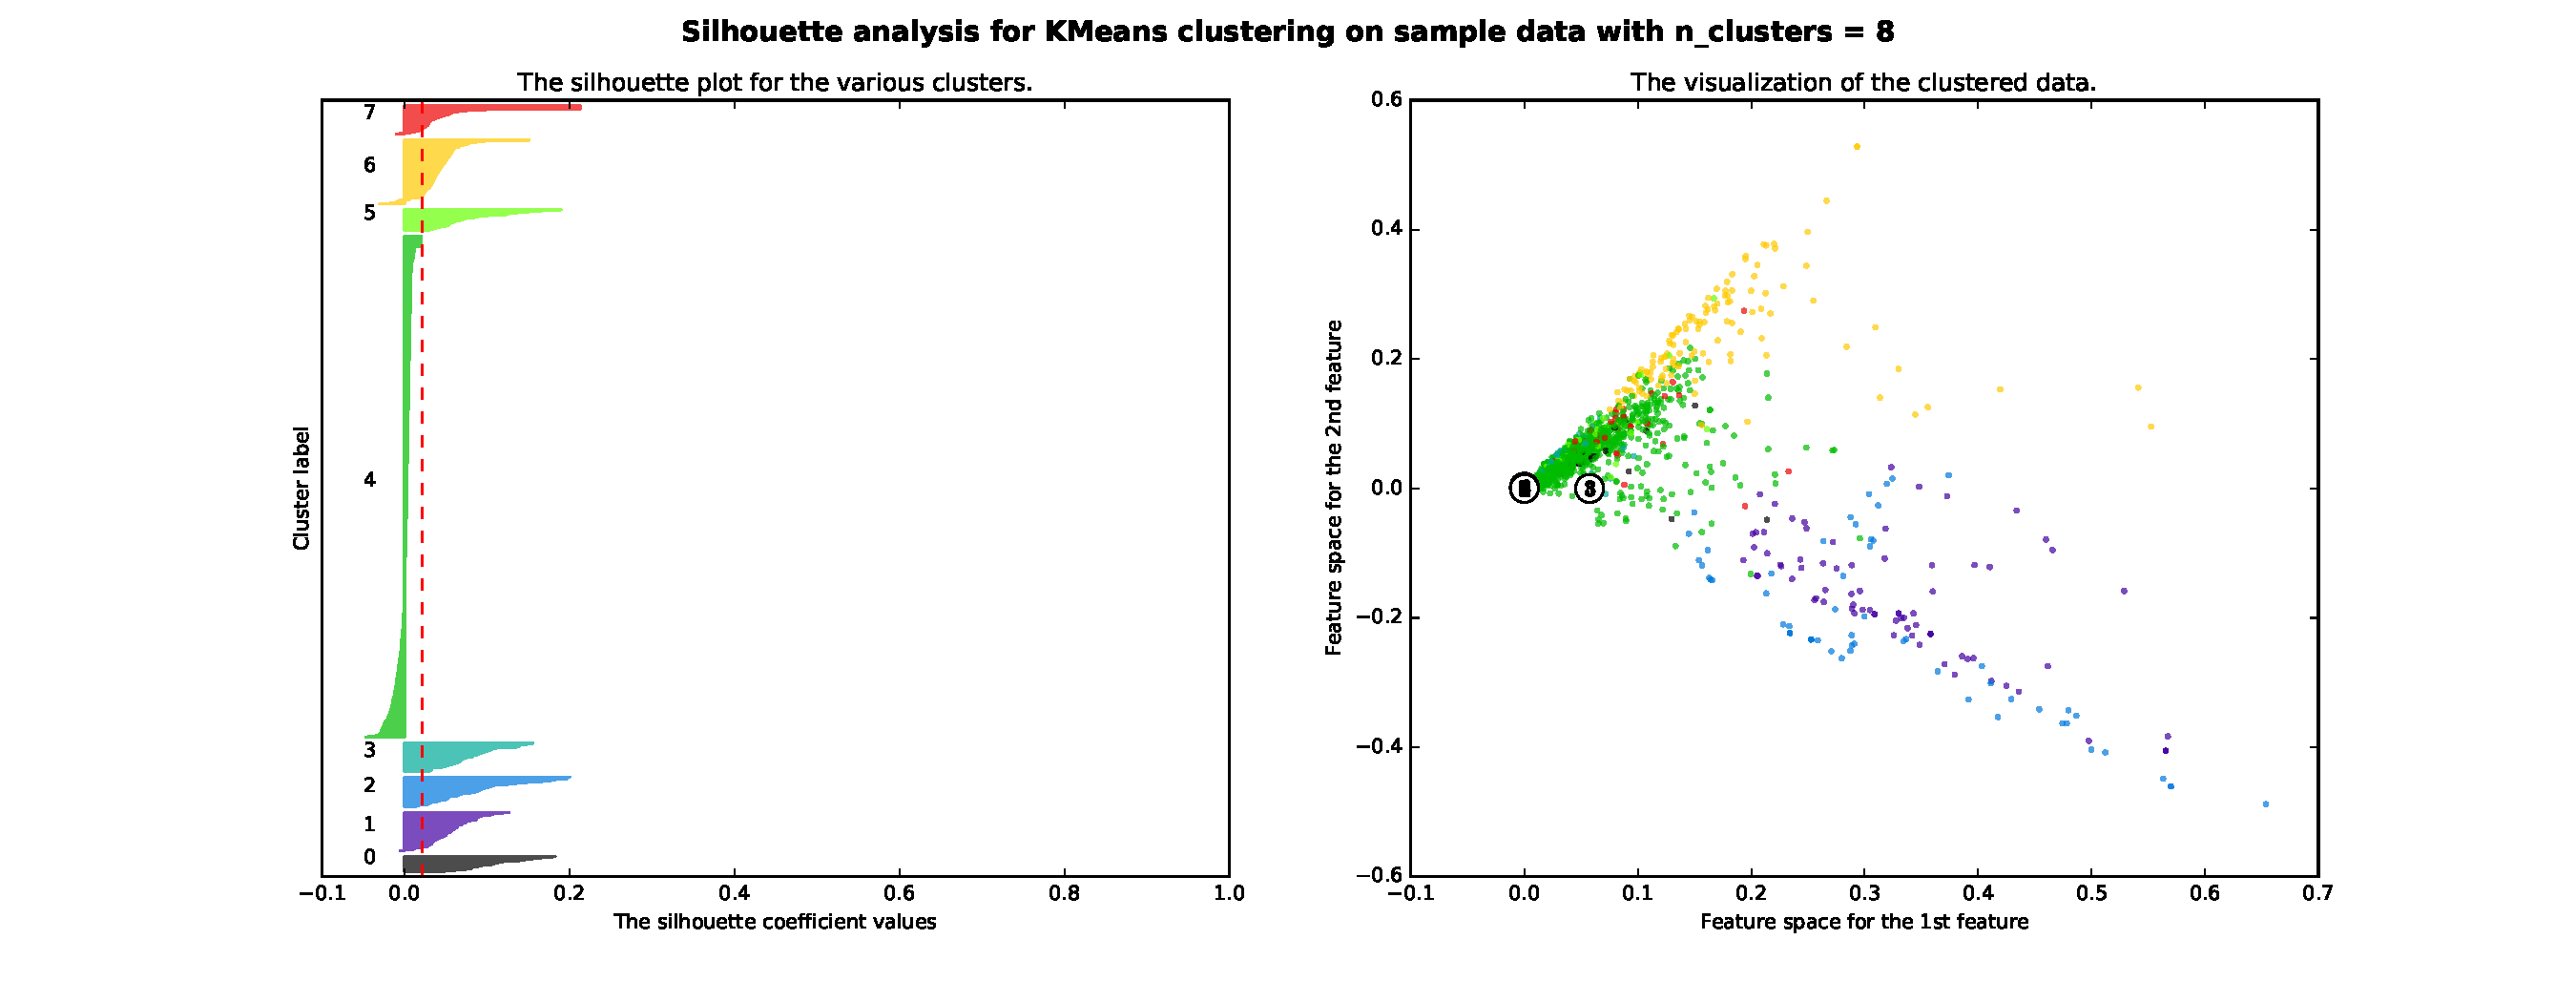
\includegraphics[width=1\textwidth]{img/exp-multi-label-paragraphs/kmeans_n=8_pca.pdf}
        \caption{Cumulative Confidence}
\label{fig:kmeans_n=6_pca}
    \end{subfigure}
    \caption{Amount of label judgements versus label confidence of the sentence label data collected via crowdflower}
\label{fig:kmeans_pca}
\end{figure}

Thus the data was sorted into a hierarchy as a second attempt to counter disambiguate and group labels that are similar.




\paragraph{Results}
\label{par:Results}

In total 91 job ads were tagged, resulting in 379 tagged text sections and 358 tags.

- data is very varied but could be mapped to 6 big topics
- prototype somewhat works (at least when data is clustered manually)
-

\paragraph{Learnings and Conclusions}
\label{par:Learnings and Conclusions}

The main learning was that instructions must be really simple and that it helps a lot to test this in a few rounds before releasing such tool to the public. The second learning was that the competition really helped to collect a lot of data.

- it's possible but need more data to make it work
- also need to constrain more



\subsubsection{Multi-class Sentence Classification}
\label{subs:Multi-class Sentence Classification}

To help this process literature for recruiters was consulted on how to write successful job advertisements and which topics to cover. The result of this grouping can be seen in Figure~\ref{fig:job-listing-structure}


\begin{figure}[h]
  \centering
  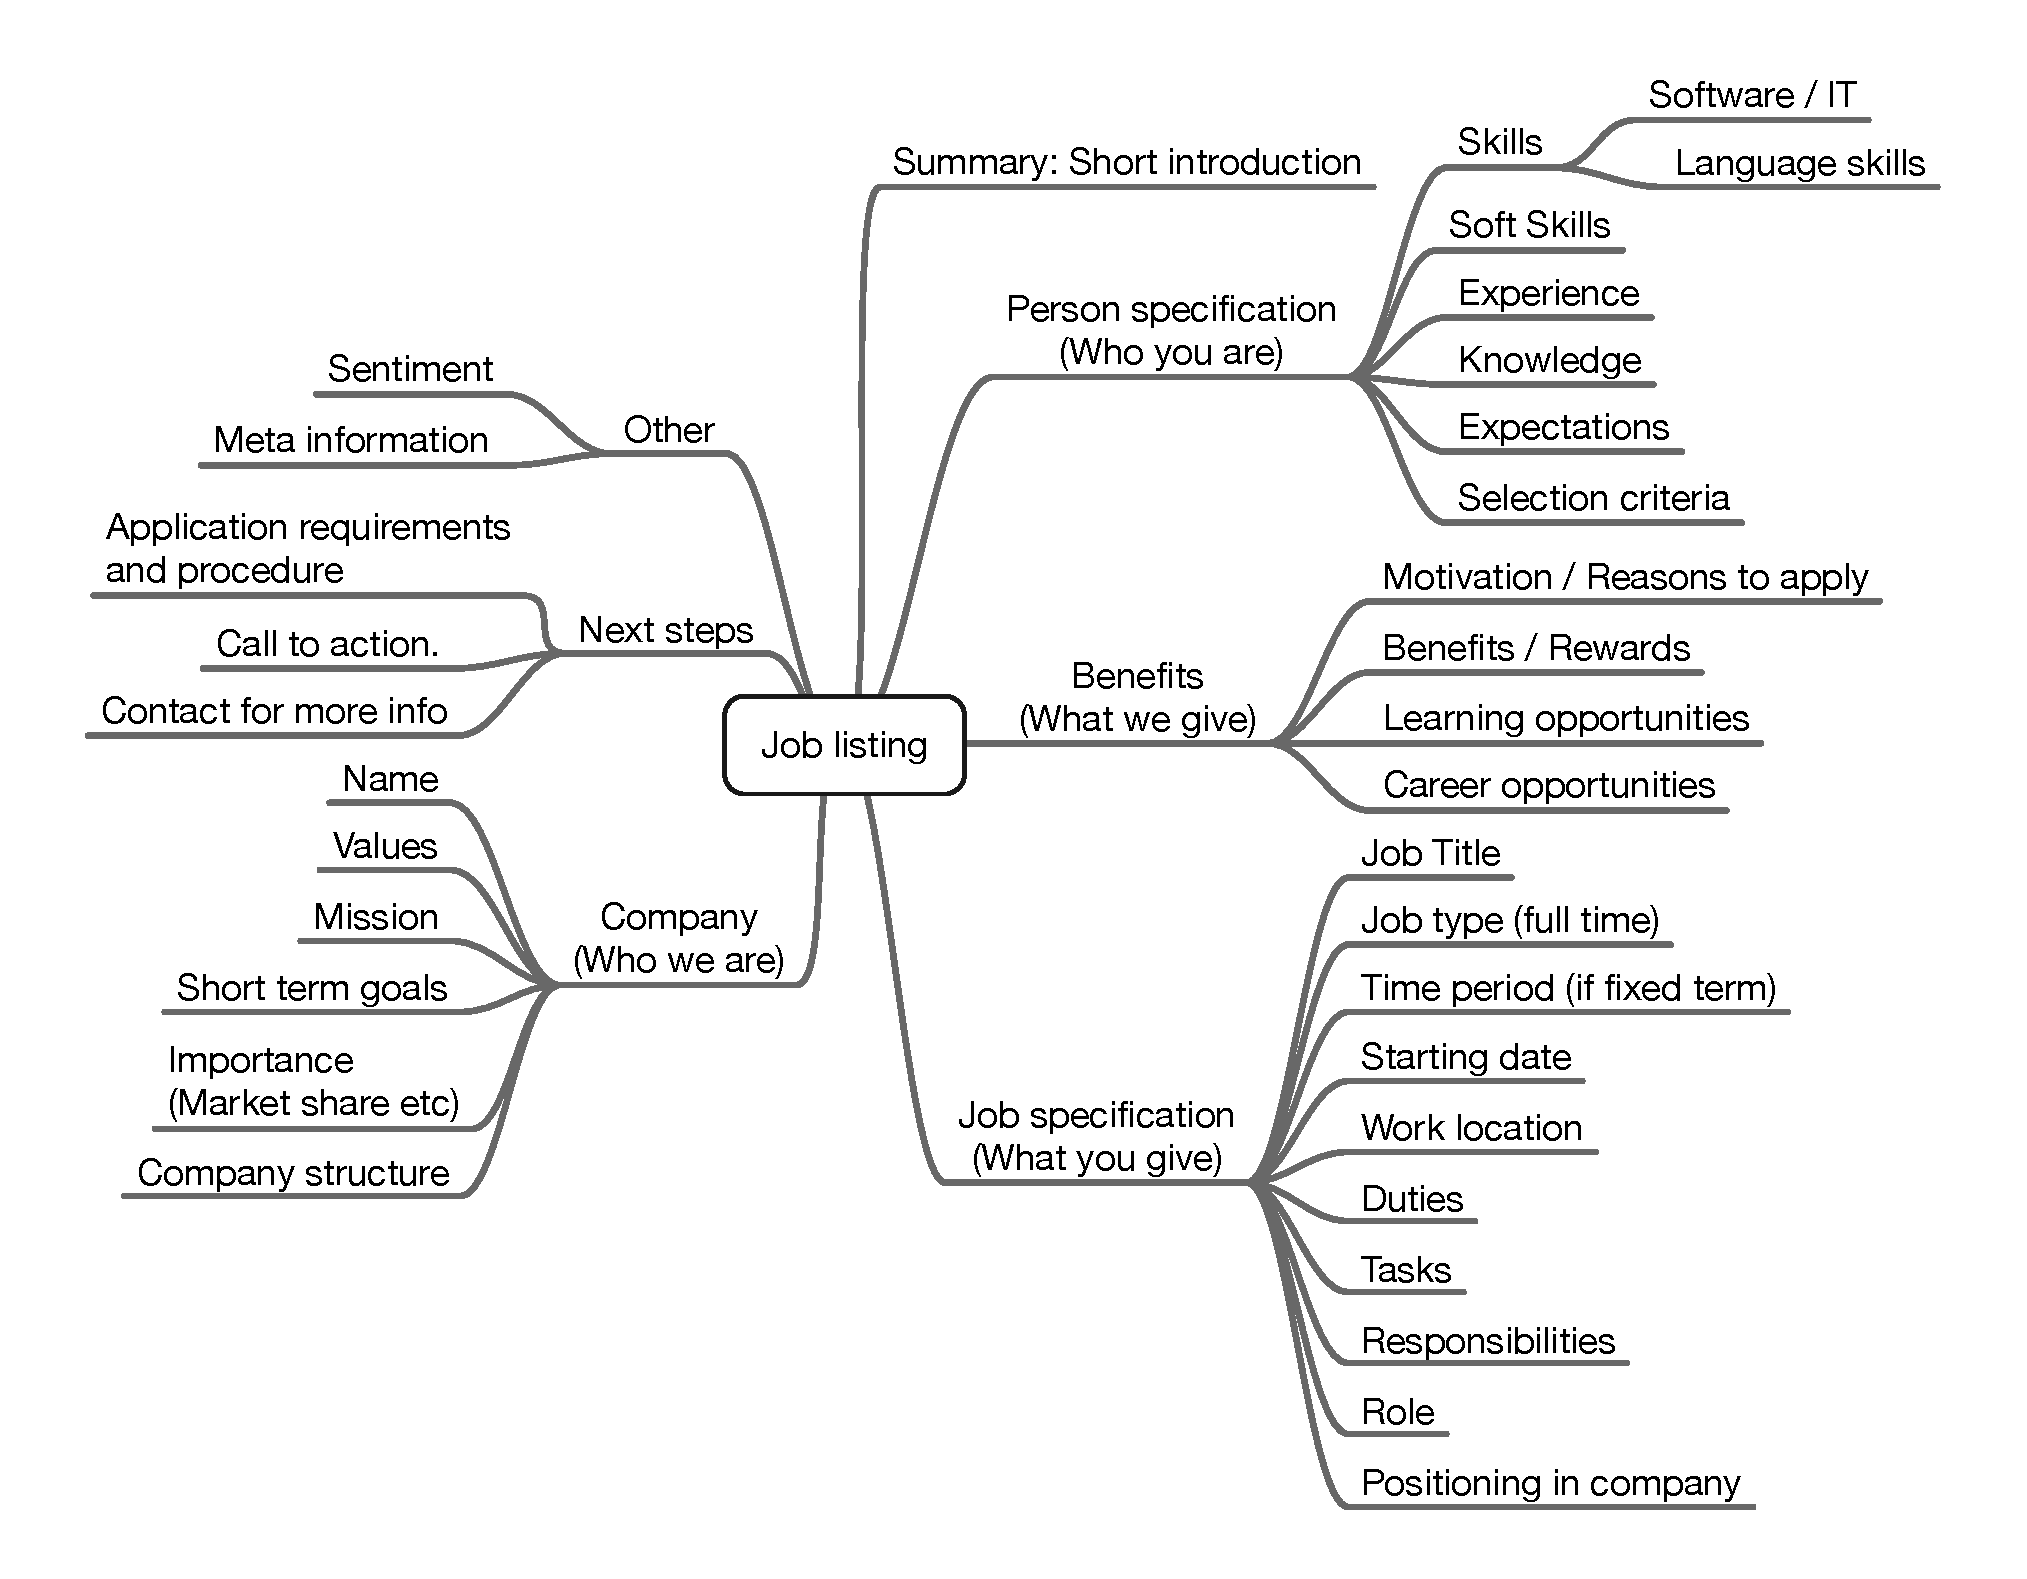
\includegraphics[width=\textwidth]{img/job-listing-structure.pdf}
  \caption{Structure of job listings inferred from the labels given by participants.}
\label{fig:job-listing-structure}
\end{figure}

\begin{figure}[h]
 % From http://localhost:8888/notebooks/thesis/experiments/vector-space-models/Vector%20Space%20Models.ipynb#Setup
    \centering
    \begin{subfigure}[b]{0.46\textwidth}
        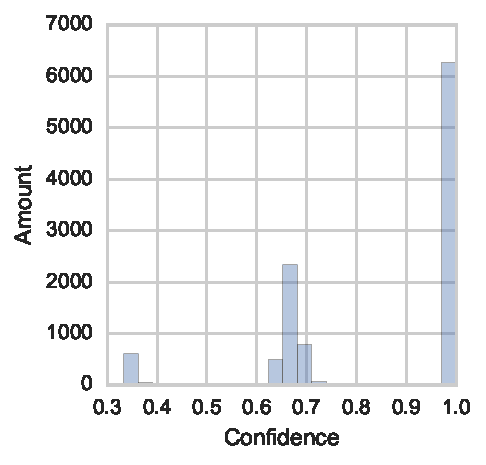
\includegraphics[width=\textwidth]{img/sentence-data-judgement-confidence.pdf}
        \caption{Confidence}
\label{fig:sentence-data-judgement-confidence}
    \end{subfigure}
~%add desired spacing between images, e. g. ~, \quad, \qquad, \hfill etc.
    %(or a blank line to force the subfigure onto a new line)
    \begin{subfigure}[b]{0.43\textwidth}
        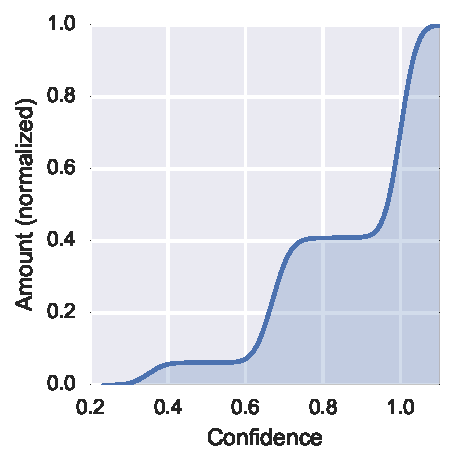
\includegraphics[width=\textwidth]{img/sentence-data-judgement-confidence-cumulative.pdf}
        \caption{Cumulative Confidence}
\label{fig:sentence-data-judgement-confidence-cumulative}
    \end{subfigure}
    \caption{Amount of label judgements versus label confidence of the sentence label data collected via crowdflower}
\label{fig:sentence-data-judgements}
\end{figure}
